\chapter{Testovanie}

\label{kap:testovanie}

Postupy popsísané v kapitole \ref{kap:identifikacia_SNP} sme implementovali v jazyku Python 3 s
výpočtovo kritickými časťami implementovanými v C++.
\todo{Odkázať na implementáciu na githube?}
V tejto kapitole náš postup testujeme na reálnych dátach.


\section{Návrh experimentu}

Na experiment budeme potrebovať dáta skladajúce sa z troch zložiek:

\begin{enumerate}
\item \label{item:reference} Postupnosť báz $A$.
\item \label{item:signal} Signál $S$ zo zariadenia MinION získaný pri sekvenovaní nejakej sekvencie $B$, 
ktorá sa od $A$ líši iba v niekoľkých SNPoch.
\item \label{item:ground} Postupnosť báz $B$, získaná nejakou presnou sekvenačnou metódou.
\end{enumerate}

Počas testovania dáme nášmu modelu na vstup iba prvé dve zložky dát, teda signál $S$ a postupnosť $A$ 
ako referenciu. Model na základe signálu odhadne, kde sa v postupnosti $B$ vyskytujú SNPy. Na základe
skutočnej postupnosti $B$ (zložka \ref{item:ground}) sa potom vyhodnotí, aká presná je predpoveď modelu.

Dáta s vhodnou štruktúrou skonštruujeme tak, že začneme so zložkami \ref{item:signal} a 
\ref{item:ground} a vytvoríme k nim zložku \ref{item:reference}. Z rôznych iných prác pracujúcich
so sekvenátorom MinION existujú dáta, kde je rovnaká DNA sekvencia osekvenovaná dvakrát: raz sekvenátorom MinION a raz nejakou 
presnou metódou. Signál zo sekvenovania prístrojom MinION môžeme teda použiť ako $S$ a výsledok presného 
sekvenovania ako $B$. Postupnosť $A$ potom vytvoríme z postupnosti $B$ tak, že v nej umelo vytvoríme
niekoľko SNPov. Takýto postup nám dáva plnú kontrolu nad množstvom SNPov, v ktorých sa $B$ líši od $A$,
nášmu modelu teda dokážeme dať na vstup dobré apriórne pravdepodobnosti.

Pri každom experimente si určíme podiel SNPov $p$, ktorý chceme mať v našich dátach. Pri konštrukcii
postupnosti $A$ postupujeme tak, že pre každú bázu postupnosti $B$ sa nezávisle rozhodneme, či ju
zmeníme. S pravdepodobnosťou $1-p$ bázu ponecháme, s pravdepodobnosťou $p$ ju zmeníme na inú, pričom
každá z troch možných iných báz má rovnakú pravdepodobnosť $\nicefrac{p}{3}$.


V každom experimente testujeme náš model s rovnakými parametrami na viacerých čítaniach. Všetky čítania
sú zo sekvenovania rovnakej postupnosti $B$, postupnosť $A$ však ku každému čítaniu vytvoríme zvlášť.
Podiel SNPov $p$ je pre všetky čítania rovnaký a dávame ho modelu k dispozícii, aby si na základe
neho vypočítal apriórne pravdepodobnosti.

Pri experimentoch používame podmnožinu dát použitých v \cite{BasecallerComparison} a podmnožinu dát z \cite{DataRondelez}.
Z týchto dát sme vytvorili osem testovacích sád s rôznymi podielmi SNPov. V každej sade bolo aj niekoľko čítaní, pri ktorých
zlyhala niektorá z prvých dvoch fáz spracovania -- buď nástroj BWA-MEM nenašiel vhodné zarovnanie čítania k referencii, alebo
nástroj \resquiggle{} nenašiel vhodné približné zarovnanie signálu k jednotlivým bázam. V tabuľke \ref{tab:datasety} uvádzame
základné charakteristiky testovacích sád.

\begin{table}[t]
\centering
\caption{Testovacie sady}
\label{tab:datasety}
\begin{tabular}{llrrrr}
\hline
skratka   & zdroj           &  čítaní & po fáze 2 & priemerná dĺžka & podiel SNPov \\ \hline
KLEBS\_01 & \cite{BasecallerComparison} & $1\,000$         & $668$                    & $18\,029$                   & $0,1 \%$     \\
KLEBS\_03 & \cite{BasecallerComparison} & $1\,000$         & $666$                    & $17\,895$                   & $0,3 \%$     \\
KLEBS\_10 & \cite{BasecallerComparison} & $1\,000$         & $657$                    & $18\,026$                   & $1 \%$       \\
KLEBS\_30 & \cite{BasecallerComparison} & $1\,000$         & $626$                    & $18\,086$                   & $3 \%$       \\
NANO\_01  & \cite{DataRondelez}         & $1\,000$         & $934$                    & $1\,801$                    & $0,1 \%$     \\
NANO\_03  & \cite{DataRondelez}         & $1\,000$         & $934$                    & $1\,803$                    & $0,3 \%$     \\
NANO\_10  & \cite{DataRondelez}         & $1\,000$         & $928$                    & $1\,801$                    & $1 \%$       \\
NANO\_30  & \cite{DataRondelez}         & $1\,000$         & $888$                    & $1\,798$                    & $3 \%$       \\ \hline
\end{tabular}
\end{table}

\section{Metriky}

V našom modeli pri každej pozícii počítame aposteriórne pravdepodobnosti pre niekoľko hypotéz. Sčítaním
pravdepodobností pre všetky tri hypotézy hovoriace, že na danej pozícii je iná báza ako v referencii,
získame pre danú pozíciu nejaké skóre. Toto skóre vyjadruje, ako veľmi je náš model presvedčený, že na tejto pozícii je SNP. To, ako dobre tieto skóre popisujú realitu, budeme v jednotlivých experimentoch vyhodnocovať pomocou dvoch metrík: krivky ROC a úspešnosti identifikácie.

\subsection{Krivka ROC}

Náš model môžeme chápať ako klasifikátor, ktorý sa snaží pozície sekvenovanej postupnosti rozdeliť
na dve skupiny: tie, na ktorých je SNP a tie, na ktorých nie je SNP.
Presnosť klasifikátorov s dvoma triedami sa často vyjadruje pomocou krivky \emph{Receiver operating characteristic} (ROC) \cite{ROC}.

Pozície, ktoré prehlásime za SNPy, môžeme vyberať pomocou prahu. Zvolíme si nejaký prah $t$ a za
SNPy budeme považovať práve tie pozície, ktoré majú skóre aspoň $t$. Voľba prahu bude ovplyvňovať,
koľkých a akých chýb sa pri klasifikácii dopustíme.
Pre každú možnú hodnotu prahu nás budú zaujímať dve čísla: \emph{Frekvencia skutočných pozitívnych príkladov} 
 a \emph{Frekvencia falošných pozitívnych príkladov}. 

\begin{definicia} 
\leavevmode
\begin{description}
\item[Frekvencia skutočných pozitívnych príkladov (TP\footnotemark)] \footnotetext{z anglického \emph{\textbf{t}rue \textbf{p}ositive}} 
je pomer počtu SNPov, \\ ktoré náš model správne označí ako SNPy, k počtu všetkých SNPov v sekvenovanej postupnosti.
\item[Frekvencia falošných pozitívnych príkladov (FP\footnotemark)] \footnotetext{z anglického \emph{\textbf{f}alse \textbf{p}ositive}} 
je pomer počtu
pozícií, ktoré náš model nesprávne označí ako SNPy, k počtu všetkých pozícií, ktoré nie sú SNPy.
\end{description}
\end{definicia}

Zvolením vhodného prahu vieme dosiahnuť ľubovoľné FP medzi $0$ a $1$, za znižovanie FP však musíme
platiť znižovaním TP. Krivka ROC je graf závislosti TP od FP. 

\todo{obrázok: príklad krivky ROC}

Čím presnejší je model, tým bližšie je jeho krivka k ľavému hornému rohu grafu (teda k bodu $
\mathrm{FP} = 0, \mathrm{TP} = 1$).
Krivka ROC pre model, ktorý ignoruje dáta a všetkým pozíciám priradí náhodné skóre, vyzerá ako diagonála
$\mathrm{TP} = \mathrm{FP}$.

Keď počítame krivky ROC pre naše experimenty, vždy uvažujeme rovnaký prah pre všetky čítania v danom 
experimente. Neuvažujeme teda možnosť, že by sme v rôznych čítaniach v rámci jedného experimentu použili 
rôzny prah.

\subsection{Úspešnosť identifikácie}

Pri identifikácii je náš hlavný cieľ trochu iný, než správne pre čo najviac pozícií určiť, či ide o SNPy. Skôr
je naším cieľom nájsť medzi všetkými pozíciami tých zopár, ktoré obsahujú SNPy. Tento cieľ sa snažíme 
reflektovať zavedením druhej metriky, ktorú nazývame \emph{úspešnosť identifikácie}. Úspešnosť identifikácie
meriame pre každé čítanie zvlášť.

\begin{definicia}
Nech $s$ je počet pozícií v čítaní, na ktorých je SNP. Nech $i$ je počet SNPov, ktoré patria medzi $s$ pozícií
s najvyšším skóre. \emph{Úspešnosť identifikácie} pre dané čítanie definujeme ako podiel $\nicefrac{i}{s}$.
\end{definicia}

Úspešnosť identifikácie je teda jedno číslo z rozsahu $0$ až $1$. Úspešnosť identifikácie je menej robustná,
než krivka ROC. V čítaniach, kde je väčší podiel SNPov, môžeme pri použití rovnakého modelu očakávať vyššiu úspešnosť identifikácie.
V extrémnom prípade, keď sú na všetkých pozíciách SNPy, bude mať ľubovoľný model úspešnosť identifikácie $1$.

Ak podiel SNPov v čítaní označíme ako $p$, úspešnosť identifikácie je rovná hodnote TP v bode, 
kde $\mathrm{TP} \cdot p + \mathrm{FP} \cdot (1-p) = p$. Tento bod sa na krivke ROC typicky nachádza v časti s
veľmi malým FP.

Pri vyhodnocovaní experimentu vypočítame úspešnosť identifikácie pre každé čítanie. Z týchto úspešností potom vypočítame
vážený priemer, kde váha každého čítania je počet SNPov v ňom. Okrem tohto priemeru uvádzame aj distribúciu 
úspešnosti identifikácie pre jednotlivé čítania.


\section{Výsledky}

\subsection[Porovnanie prístupu so štyroma hypotézami a prístupu s $3(2k-1)+1$ hypotézami]{Porovnanie prístupu so štyroma hypotézami a prístupu s $\boldsymbol{3(2k-1)+1}$ hypotézami}
\label{exp:4vsMany}
V tejto časti porovnávame verziu nášho modelu popísanú v kapitole \ref{sec:jedna_pozicia} s
verziou popísanou v kapitole \ref{sec:blizke_pozicie}.
Obe verzie nášho modelu sme pustili na testovacej sade KLEBS\_10 s parametrom $M=2$ (minimálny počet hodnôt signálu zarovnaný k jednej báze).
Vylepšenia popísané v kapitole \ref{sec:vylepsenia} zatiaľ nepoužívame.


Výsledok testovania úvádzame v grafoch na Obr. \ref{fig:grafy_4vsMany}.
Prístup s $3(2k-1)+1$ hypotézami má priemernú úspešnosť identifikácie $47,6 \%$, prístup so štyroma hypotézami má
priemernú úspešnosť $33,2 \%$.
Na krivke ROC vidíme, že prístup s $3(2k-1)+1$ hypotézami je lepší pre nízke FP, 
kým prístup so štyroma hypotézami je lepší pre vysoké TP. 
V ďalších experimentoch používame prístup s $3(2k-1)+1$ hypotézami, keďže má výrazne lepšiu úspešnosť identifikácie.

\begin{figure}[t]
\begin{subfigure}{0.5\textwidth}
\centerline{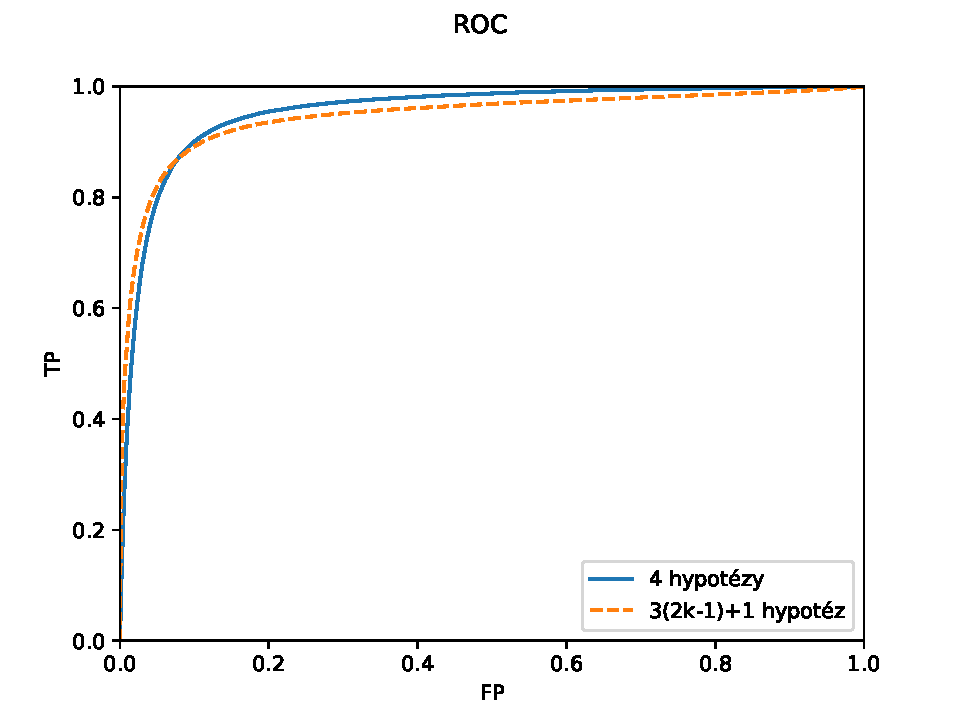
\includegraphics[width=\linewidth]{plots/1_ROC}}
\end{subfigure}%
\begin{subfigure}{0.5\textwidth}
\centerline{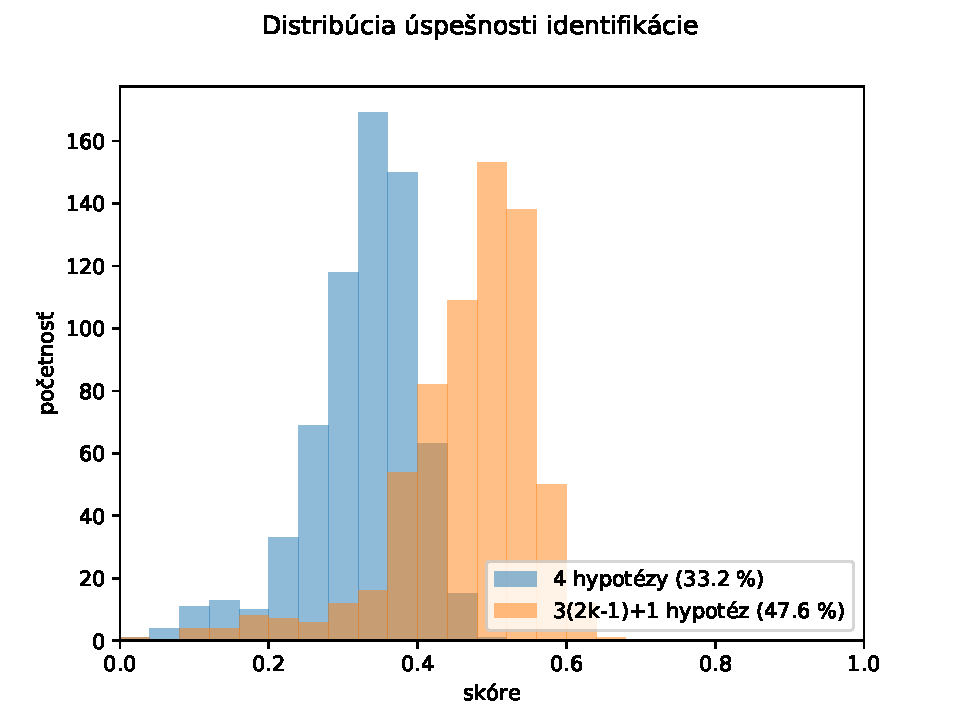
\includegraphics[width=\linewidth]{plots/1_uspesnost_eqbins}}
\end{subfigure}
\caption{Krivka ROC a distribúcia úspešnosti identifikácie pre prístup so štyroma hypotézami a pre prístup s $3(2k-1)+1$ hypotézami.}
\label{fig:grafy_4vsMany}
\end{figure}

Hlavným dôvodom zavedenia nových hypotéz bola snaha lepšie vyhodnocovať pozície blízko SNPov. 
Grafy na Obr. \ref{fig:proximity} ukazujú, že zavedením viacerých hypotéz sa dramaticky znížilo množstvo pozícií tesne vedľa SNPov s
vysokým skóre.

\begin{figure}[t]
\begin{subfigure}{0.5\textwidth}
\centerline{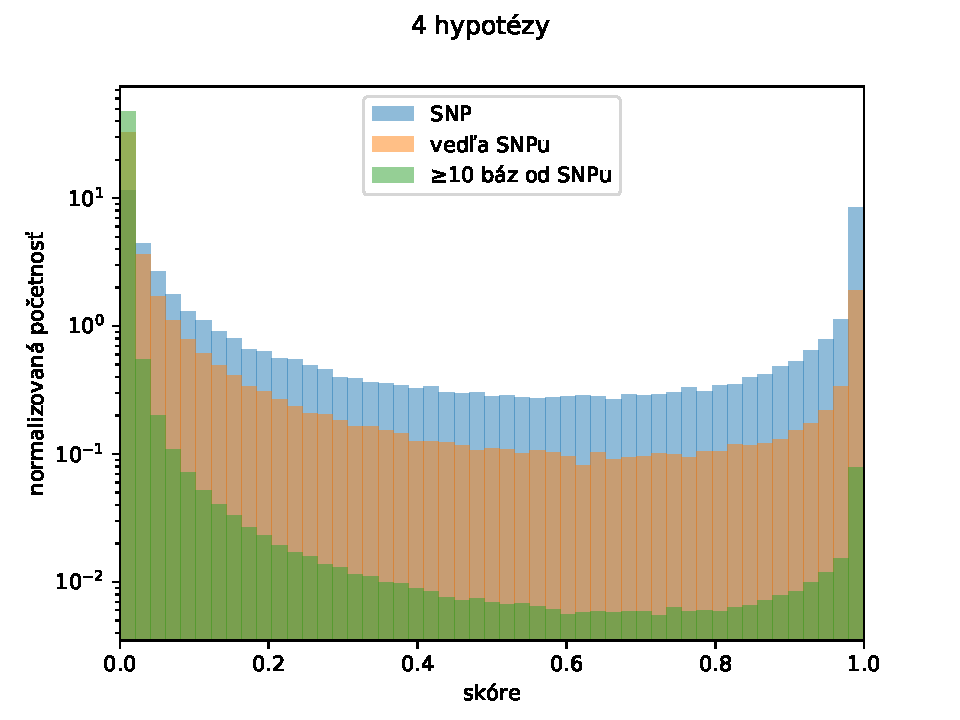
\includegraphics[width=\linewidth]{plots/1_windowed_titled_eqbins}}
\end{subfigure}%
\begin{subfigure}{0.5\textwidth}
\centerline{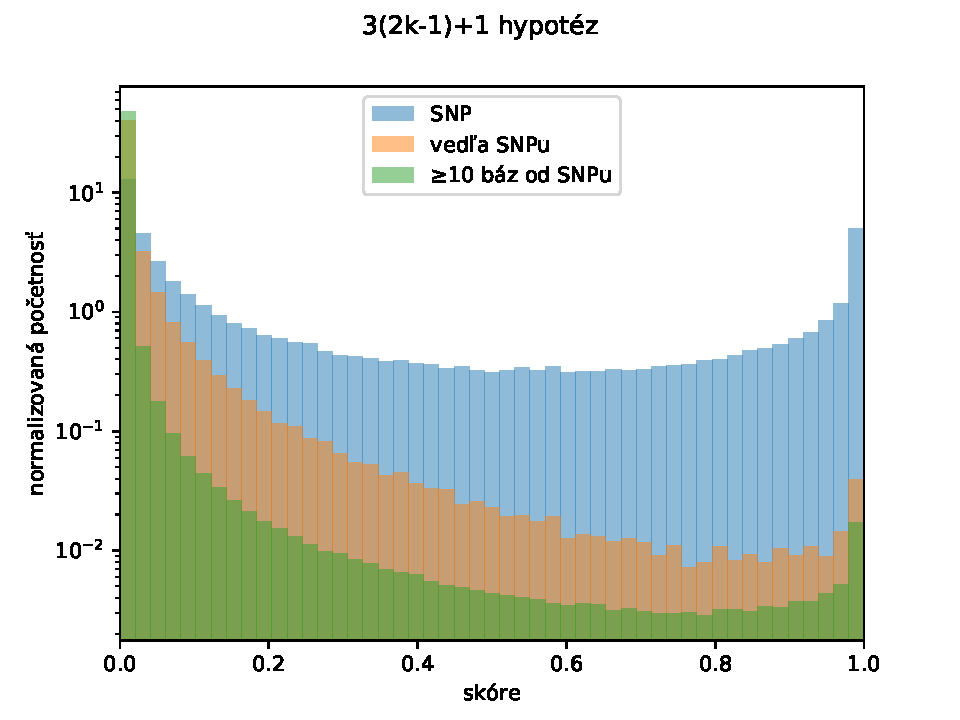
\includegraphics[width=\linewidth]{plots/1_moving_eqbins}}
\end{subfigure}
\caption{Porovnanie distribúcie skóre pre pozície so SNPom, vedľa SNPu a ďaleko od SNPov pre model s štyroma hypotézami
a model s $3(2k-1)+1$ hypotézami.}
\label{fig:proximity}
\end{figure}



\subsection{Vplyv dolaďovania normalizácie}
\label{exp:tweaking}
V tomto experimente meriamie vplyv dolaďovania normalizácie navrhovaného v kapitole \ref{upg:tweaking}. Náš model sme
dvakrát pustili na testovacej sade KLEBS\_10 : 
raz s dolaďovaním
normalizácie a raz bez neho. V oboch prípadoch používame $M=2$, modelovanie cúvania zatiaľ nepoužívame.

Výsledok testovania uvádzame v grafoch na Obr. \ref{fig:grafy_tweaking}. Bez dolaďovania normalizácie mal model priemernú
úspešnosť identifikácie $47,6 \%$, s dolaďovaním $47,8 \%$. Na krivke ROC vidíme, že pre vysoké TP je model s dolaďovaním
mierne presnejší. Keďže dolaďovanie normalizácie mierne zvýšilo presnosť modelu, v ďalších experimentoch
používame model s dolaďovaním normalizácie.

\begin{figure}[t]
\begin{subfigure}{0.5\textwidth}
\centerline{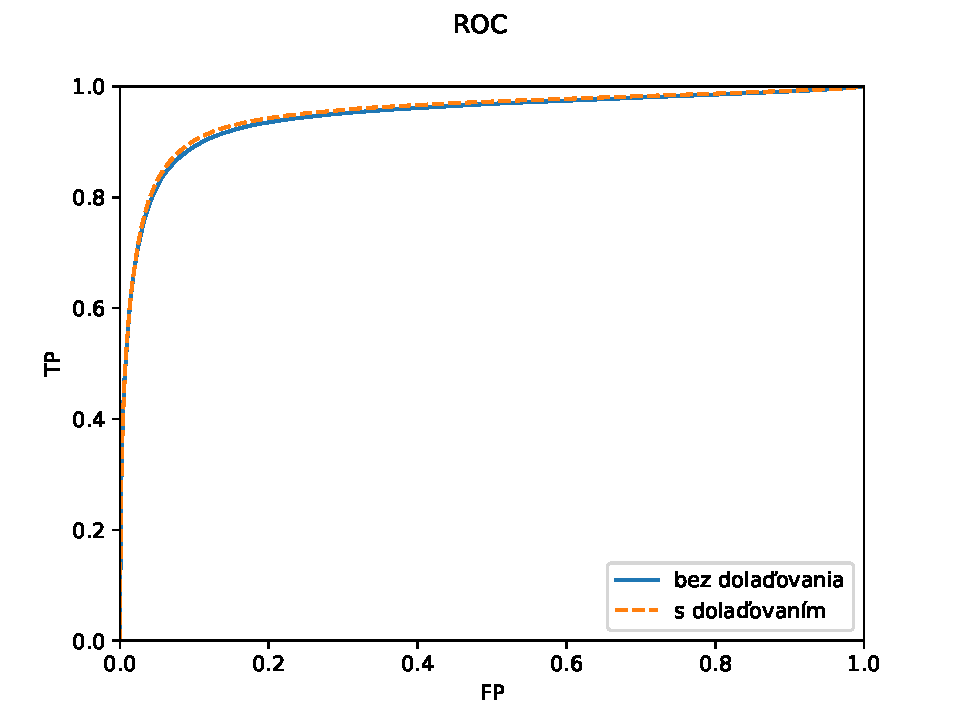
\includegraphics[width=\linewidth]{plots/2_ROC}}
\end{subfigure}%
\begin{subfigure}{0.5\textwidth}
\centerline{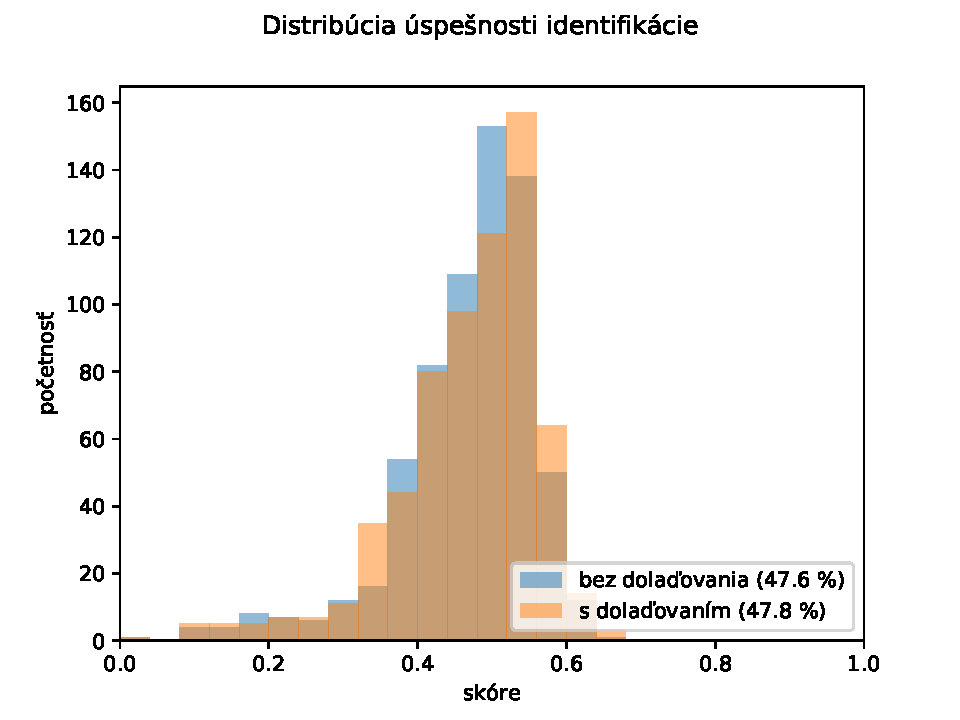
\includegraphics[width=\linewidth]{plots/2_uspesnost_eqbins}}
\end{subfigure}
\caption{Krivka ROC a distribúcia úspešnosti identifikácie bez dolaďovania normalizácie a s dolaďovaním normalizácie.}
\label{fig:grafy_tweaking}
\end{figure}

\subsection{Vplyv modelovania cúvania}
\label{exp:flashbacks}
Tento experiment skúma vplyv modelovania cúvania navrhovaného v kapitole \ref{upg:flashbacks}. Náš model sme
opäť pustili testovacej sade KLEBS\_10, raz bez modelovania cúvania a raz s ním. Opäť v oboch prípadoch používame $M=2$.

Grafy s výsledkami uvádzame na Obr. \ref{fig:grafy_flashbacks}. Bez modelovania cúvania má náš model priemernú úspešnosť
identifikácie $47,6 \%$, s modelovaním cúvania má priemernú úspešnosť $54,8 \%$.
Keďže modelovanie cúvania spresňuje náš model, v ďalších experimentoch používame model s modelovanám
cúvania.

\begin{figure}[t]
\begin{subfigure}{0.5\textwidth}
\centerline{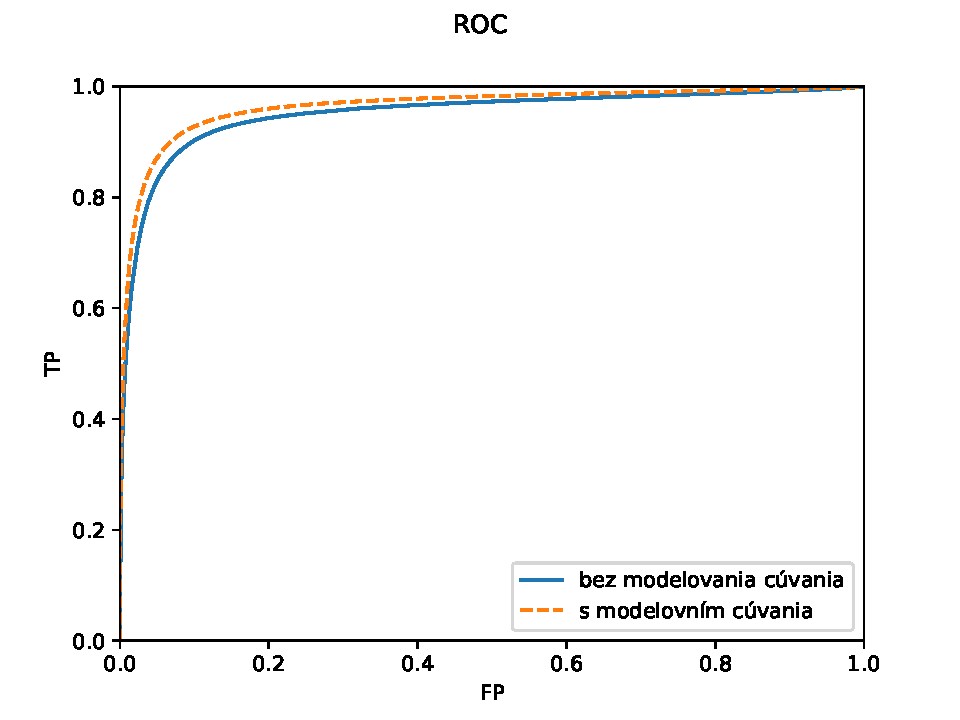
\includegraphics[width=\linewidth]{plots/3_ROC}}
\end{subfigure}%
\begin{subfigure}{0.5\textwidth}
\centerline{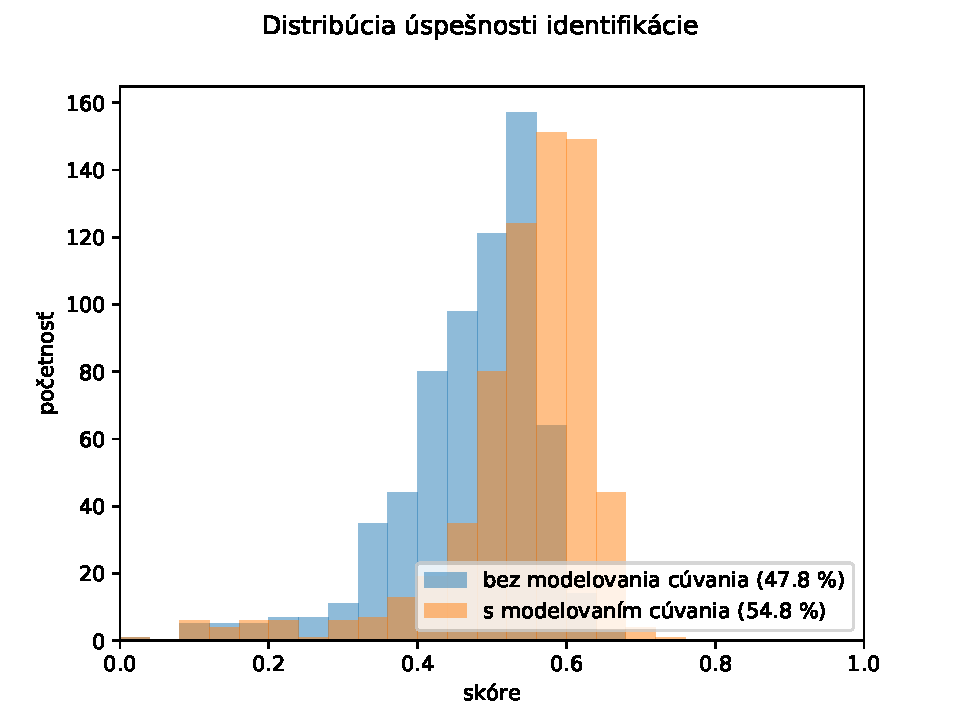
\includegraphics[width=\linewidth]{plots/3_uspesnost_eqbins}}
\end{subfigure}
\caption{Krivka ROC a distribúcia úspešnosti identifikácie bez modelovania cúvania a s modelovaním cúvania.}
\label{fig:grafy_flashbacks}
\end{figure}

\subsection[Vplyv parametra $M$]{Vplyv parametra $\boldsymbol{M}$}
V tomto experimente sme náš model pustili postupne pre $M = 1, 2, \dots, 6$. Stále používame testovaciu sadu KLEBS\_10.
Krivky ROC uvádzame na Obr. \ref{fig:ROC_M}. Priemernú úspešnosť identifikácie uvádzame v tabuľke \ref{tab:uspesnost_M}.
Vidíme, že náš model je najpresnejší pre $M=2$ a $M=3$. Zvyšovanie $M$ na $4$ a viac je už kontraproduktívne. V ďalších
experimentoch preto budeme používať iba $M=2$ a $M=3$. Distribúciu úspešnosti identifikácie pre $M = 2$ a $M = 3$ uvádzame
v grafe na Obr. \ref{fig:uspesnost_M}.

\begin{figure}[t]
\begin{subfigure}{0.5\textwidth}
\centerline{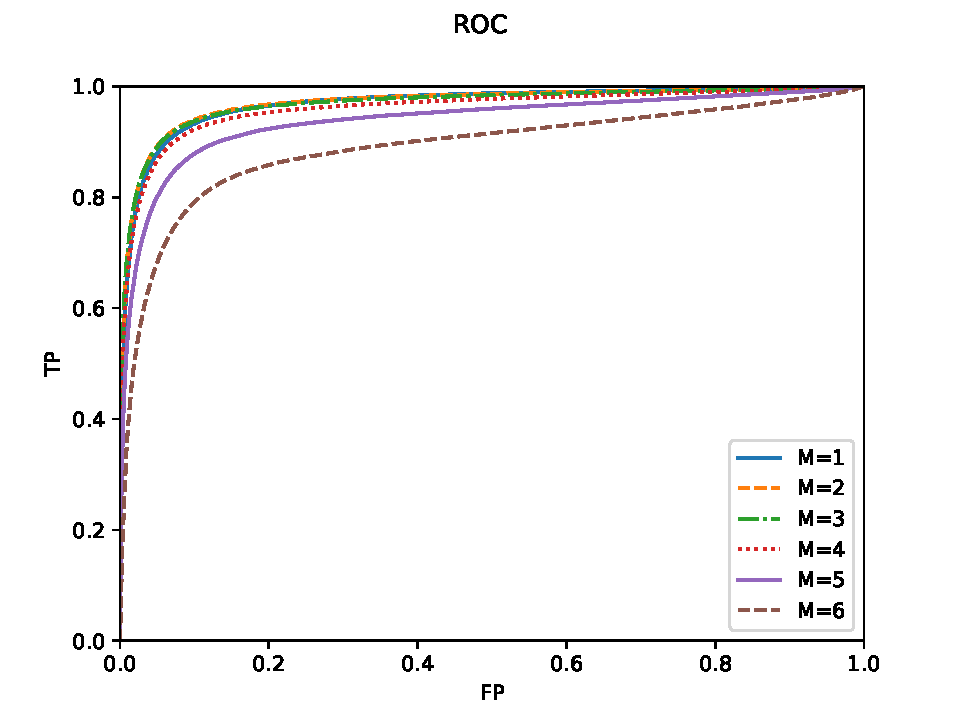
\includegraphics[width=\linewidth]{plots/4_ROC}}
\end{subfigure}%
\begin{subfigure}{0.5\textwidth}
\centerline{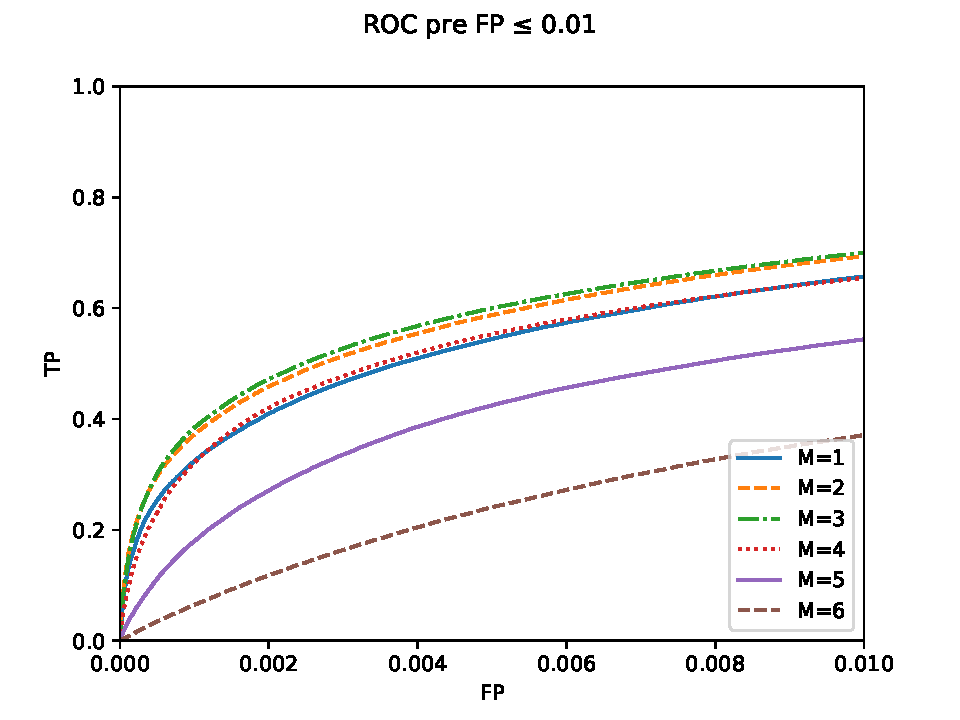
\includegraphics[width=\linewidth]{plots/4_ROC_zoom}}
\end{subfigure}
\caption{Krivka ROC pre $M = 1, 2, \dots, 6$. Graf vpravo zobrazuje časť kriviek pre $\mathrm{FP} \leq 0,01$.}
\label{fig:ROC_M}
\end{figure}

\begin{figure}[t]
\centerline{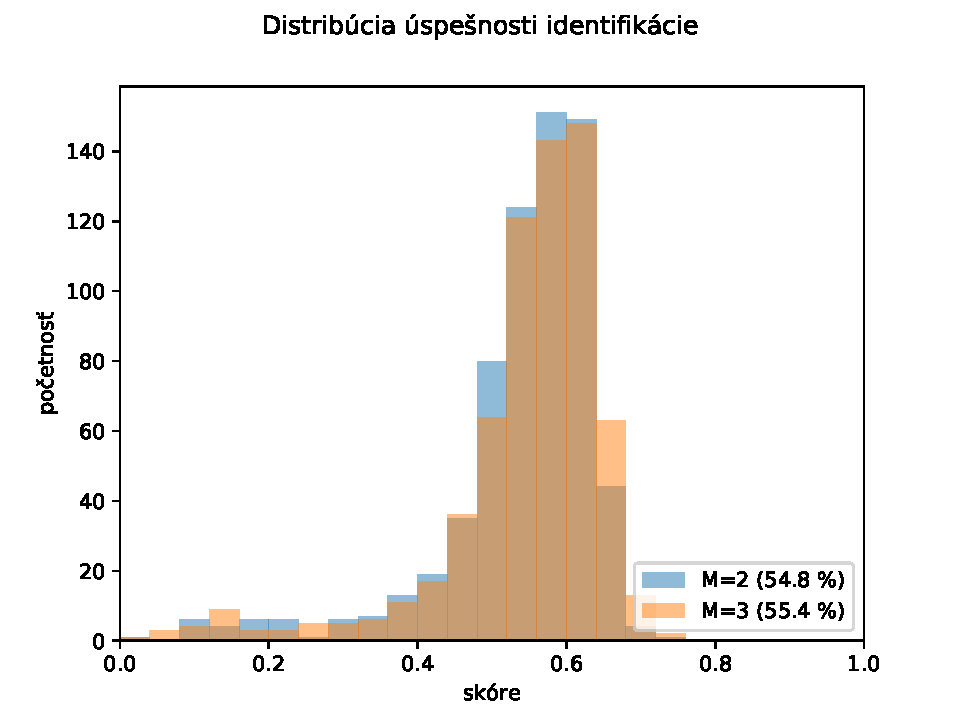
\includegraphics[width=0.5\textwidth]{plots/4_uspesnost_1az2}}
\caption{Distribúcia úspešnosti identifikácie pre $M = 2$ a $M = 3$.}
\label{fig:uspesnost_M}
\end{figure}

\begin{table}[t]
\centering
\caption{Priemerná úspešnosť identifikácie pre rôzne $M$}
\label{my-label}
\begin{tabular}{lrrrrrr}
\hline
$M$                       & 1         & 2         & 3         & 4         & 5         & 6         \\ \hline
úspešnosť identifikácie & $54,3 \%$ & $57,4 \%$ & $58,1 \%$ & $54,5 \%$ & $45,7 \%$ & $33,6 \%$ \\ \hline
\end{tabular}
\label{tab:uspesnost_M}
\end{table}


\subsection{Porovnanie s priamočiarym prístupom}

K identifikácii variantov sa dá pristupovať aj priamočiarejšie, než k nej pristupuje náš model:
zo signálu by sme mohli pomocou basecallera určiť bázy a následne hľadať rozdiely medzi postupnosťou
báz z basecallera a referenciou.

V našej práci sme sa snažili navrhnúť model, ktorý by bol presnejší, než takýto priamočiary
prístup. V tejto časti preto navrhneme, ako identifikovať SNPy len na základe referencie a postupnosti
báz, ktorú zo signálu vypočíta basecaller. Tento postup potom porovnáme s naším modelom.

\subsubsection{Priamočiary prístup}

Postupnosť báz, ktorú nám dá basecaller, budeme volať \emph{vzorka}. Keďže basecaller nevie,
akú dlhú postupnosť sme sekvenovali, dĺžka vzorky sa nemusí zhodovať s dĺžkou 
zodpovedajúcej časti referencie.
Na niektorých miestach basecaller nájde viac báz, než tam reálne je, na iných zasa niektoré
bázy nenájde.

Na začiatku preto vzorku pomocou nástroja BWA-MEM zarovnáme k referencii. 
Toto zarovnanie nám určuje, ktoré časti referencie a vzorky si vzájomne zodpovedajú, pričom
niektoré pozície z referencie nemusia zodpovedať žiadnym pozíciám zo vzorky, a obrátene. Zarovnanie v podstate hovorí, ktoré časti referencie 
a ktoré časti vzorky treba vynechať, aby k sebe to, čo zostane, čo najlepšie pasovalo. 

\todo{obrázok: dve zarovnané DNA postupnosti}

Na základe
tohto zarovnaia rozdelíme pozície v referencii na štyri skupiny:

\begin{description}

\item[Delécie.] Pozície v referencii, ktorým nezodpovedá žiadna pozícia zo vzorky.
\item[Substitúcie.] Pozície v referencii, kde sa báza z referencie líši od zodpovedajúcej
bázy vo vzorke.
\item[Blízko inzercií.] Pozície v referencii, ktorých zodpovedajúca pozícia vo vzorke susedí
s časťou vzorky, ktorá nezodpovedá ničomu v referencii. Budeme pritom vyžadovať, aby nešlo
o substitúcie.
\item[Zhody:] Pozície, kde sa báza v referencii zhoduje s bázou vo vzorke a nie sú blízko inzercií.

\end{description}

Podobne ako pri pravdepodobnostnom modeli, každej pozícii priradíme skóre vyjadrujúce,
ako veľmi si myslíme, že ide o SNP. Toto skóre bude závisieť iba od toho, do ktorej zo štyroch skupín
daná pozícia patrí. Budú teda existovať iba štyri možné hodnoty skóre, krivka ROC pre tento prístup
teda bude mať iba 5 bodov (pričom jeden z nich bude $\mathrm{TP} = 0, \mathrm{FP} = 0$ a
jeden bude $\mathrm{TP} = 1, \mathrm{FP} = 1$).

Tieto štyri možné hodnoty skóre určujeme nasledujúcim spôsobom. Na niekoľkých trénovacích čítaniach
sme pre každú zo štyroch skupín $G$ odmerali, aká časť všetkých pozícií, na ktorých je SNP, patrí do skupiny $G$ 
(toto číslo označme $V(G)$)
 a aká časť všetkých pozícií bez SNPu patrí do skupiny $G$ (toto číslo označme $N(G)$). 
Hodnotu $V(G)$ používame ako podmienenú pravdepodobnosť, že by pozícia so SNPom bola v skupine $G$
a hodnotu $N(G)$ používame ako podmienenú pravdepodobnosť, že by pozícia bez variantu bola v skupine 
$G$. Pre každú pozíciu potom na základe týchto podmienených pravdepodobností a apriórnej 
pravdepodobnosti, že na danej pozícii je SNP, vypočítame aposteriórnu pravdepodobnosť, že je na tejto
pozícii SNP. Táto aposteriórna pravdepodobnosti bude skóre pre danú pozíciu.

\subsection{Experimenty}

Priamočiary prístup porovnávame s naším modelom pre $M=2$ a $M=3$ na všetkých ôsmich testovacích sadách.
Pri vyhodnocovaní úspešnosti identifikácie priamočiareho prístupu sa nám stáva, že nevieme jednoznačne
vybrať $s$ pozícií s najvyšším skóre, pretože veľa pozícií má rovnaké skóre. V takých prípadoch spomedzi
kandidátov s rovnako vysokým skóre vyberáme náhodne. Krivky ROC uvádzame v grafe na Obr. \ref{fig:ROC_final}.
Priemerné úspešnosti identifikácie uvádzame v tabuľke \ref{tab:uspesnost_final}. Distribúcie úspešnosti
identifikácie uvádzame na Obr. \ref{fig:uspesnost_final}.
 
 
\begin{figure}[!ht]
   \begin{center}
   \begin{minipage}{\textwidth}
     \centering
     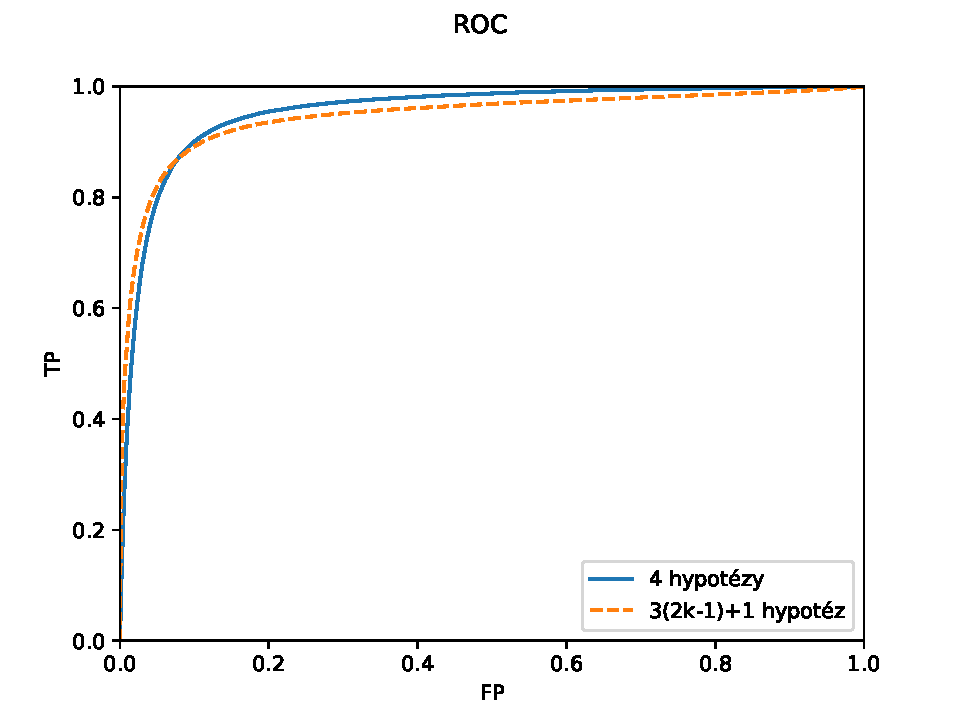
\includegraphics[width=.47\textwidth]{plots/1_ROC}\quad
     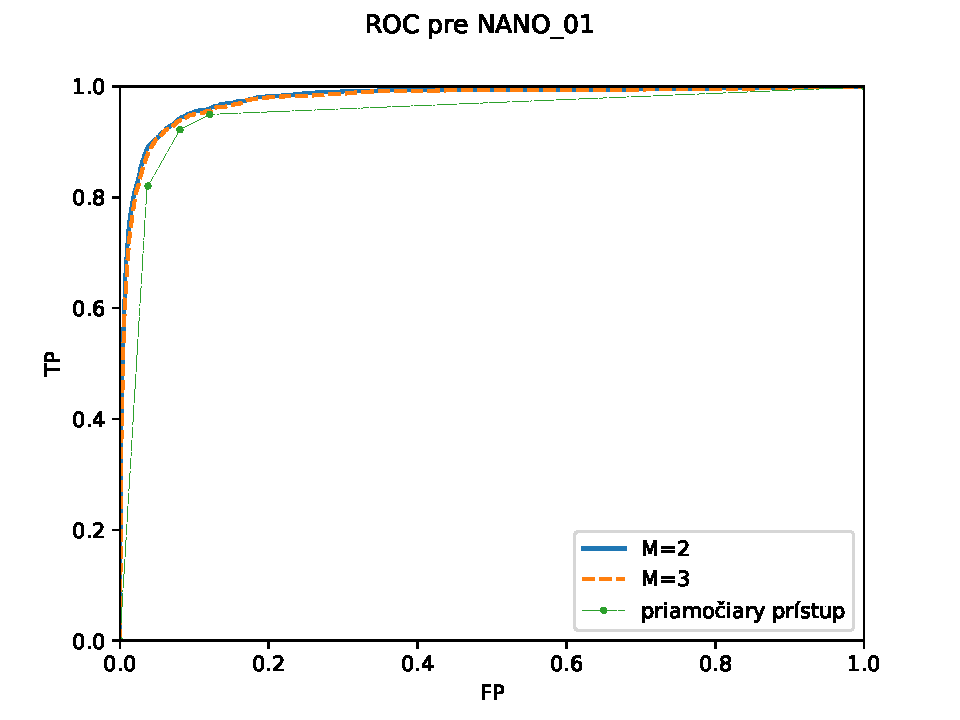
\includegraphics[width=.47\textwidth]{plots/6_ROC_nanolution_01}\\
     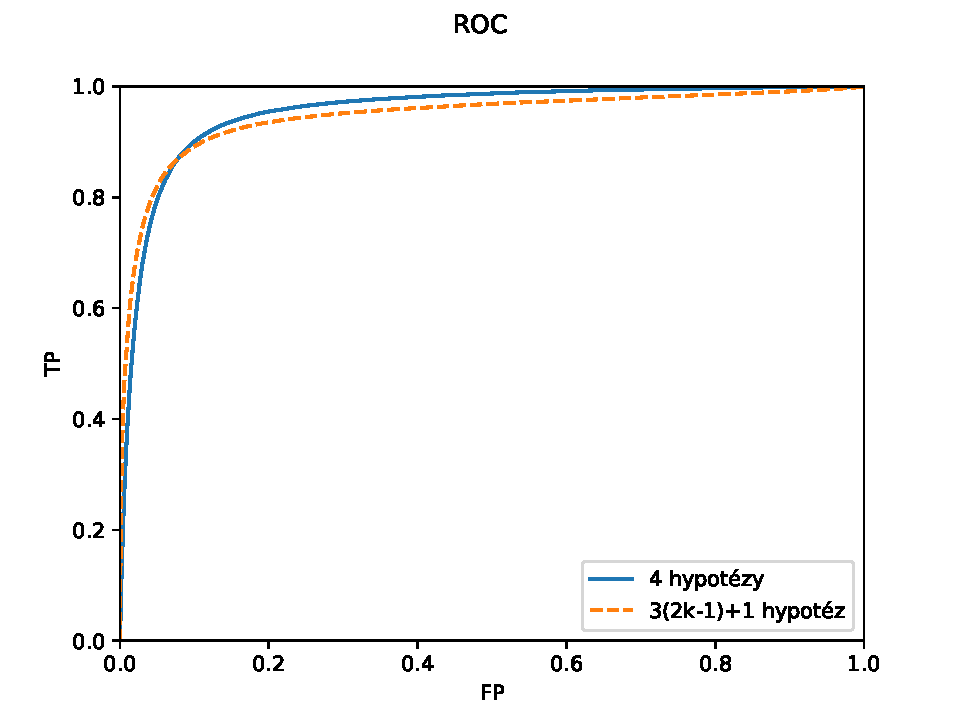
\includegraphics[width=.47\textwidth]{plots/1_ROC}\quad
     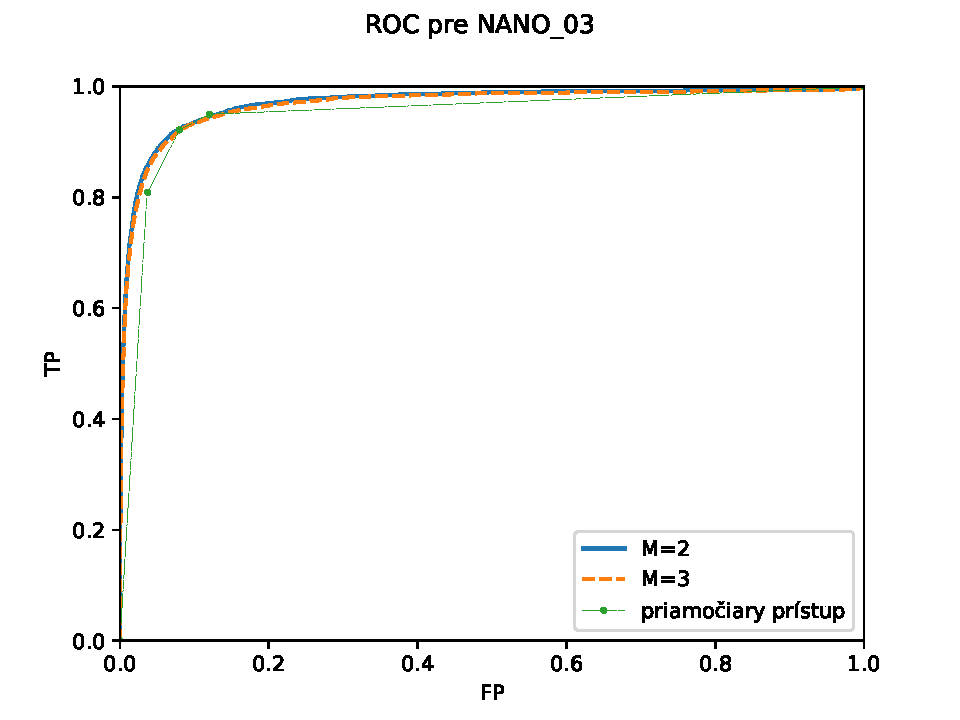
\includegraphics[width=.47\textwidth]{plots/6_ROC_nanolution_03}\\
     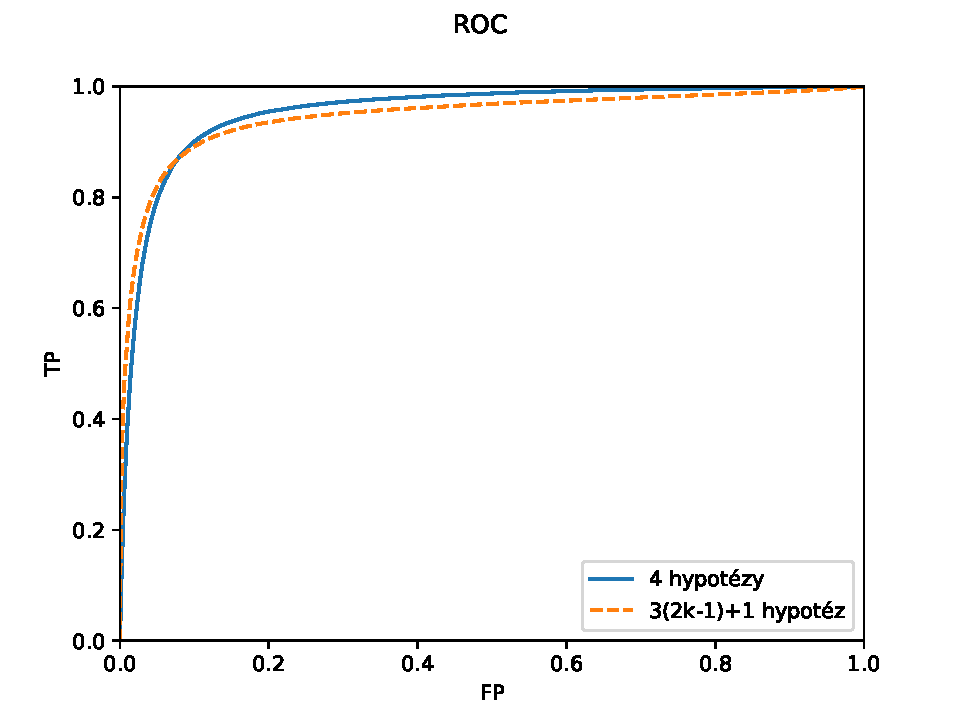
\includegraphics[width=.47\textwidth]{plots/1_ROC}\quad
     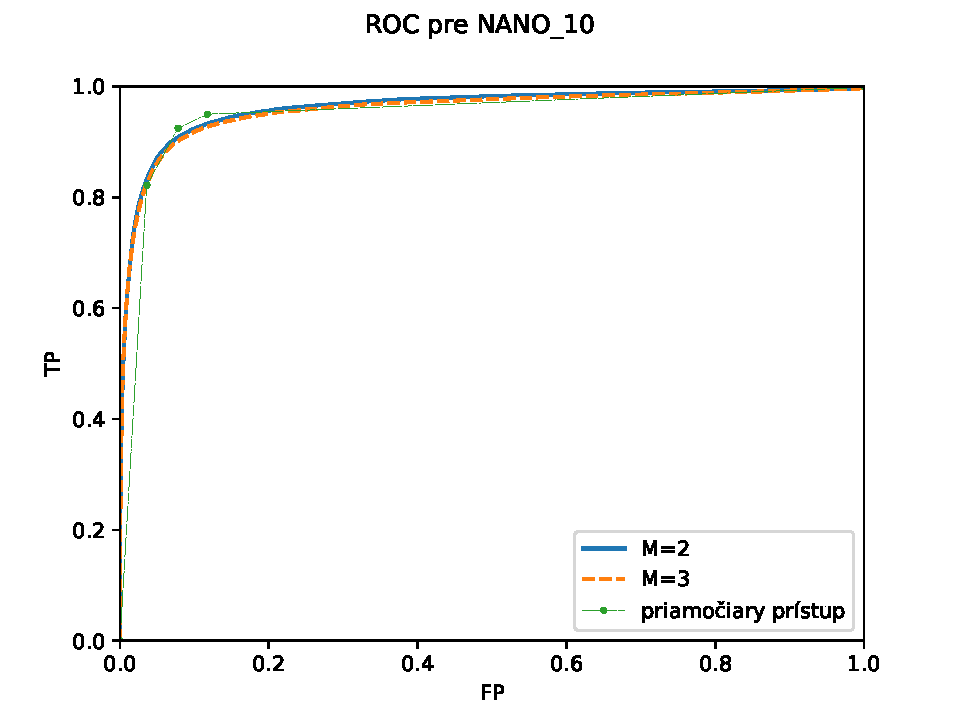
\includegraphics[width=.47\textwidth]{plots/6_ROC_nanolution_10}\\
     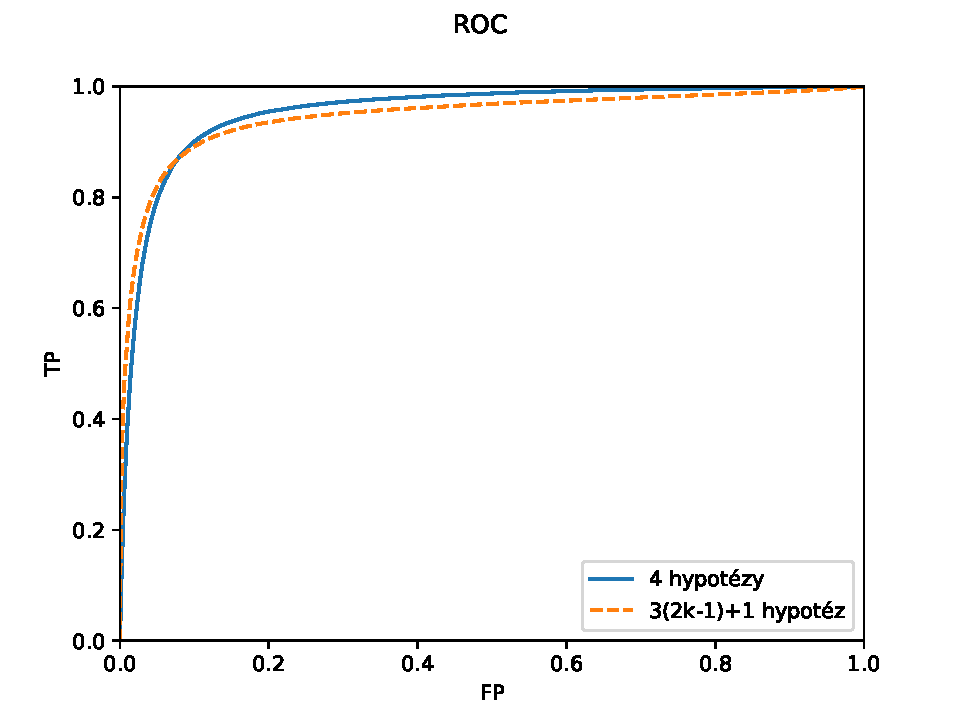
\includegraphics[width=.47\textwidth]{plots/1_ROC}\quad
     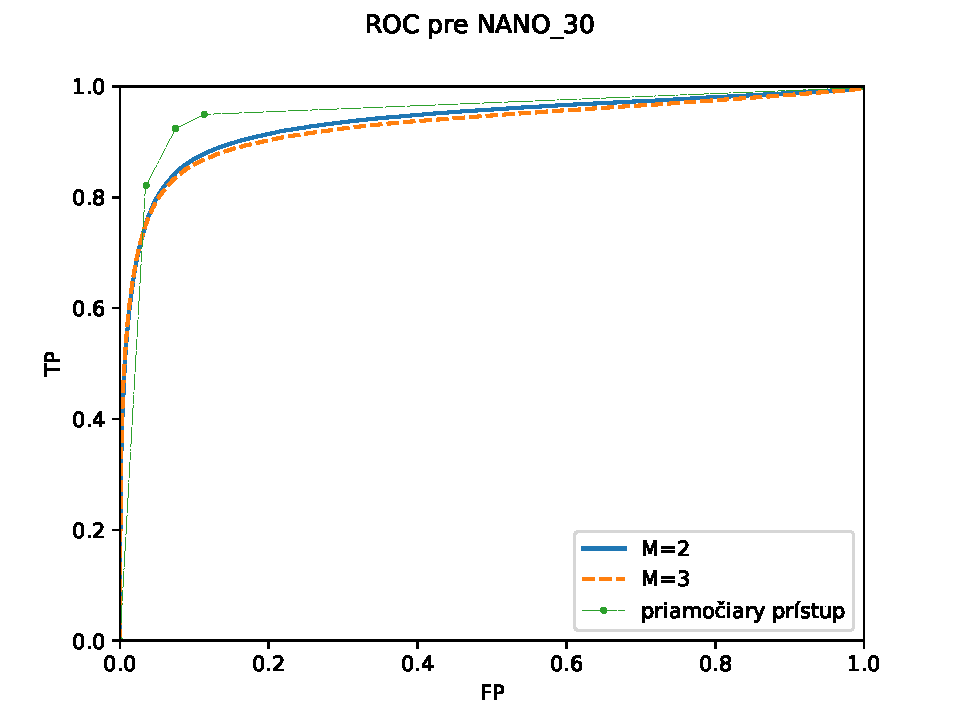
\includegraphics[width=.47\textwidth]{plots/6_ROC_nanolution_30}
   \end{minipage}\\[1em]   
   \end{center}
\caption{Krivky ROC pre priamočiary prístup a pre náš model s $M=2$ a $M=3$.}
\label{fig:ROC_final}
\end{figure}
 
\begin{figure}[!ht]
   \begin{center}
   \begin{minipage}{\textwidth}
     \centering
     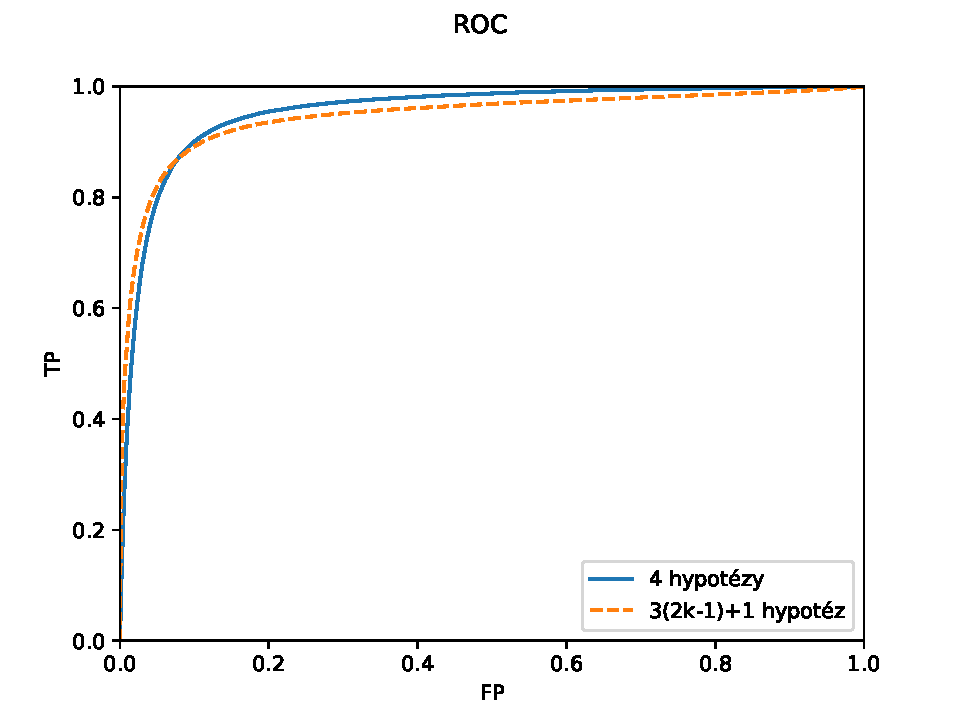
\includegraphics[width=.47\textwidth]{plots/1_ROC}\quad
     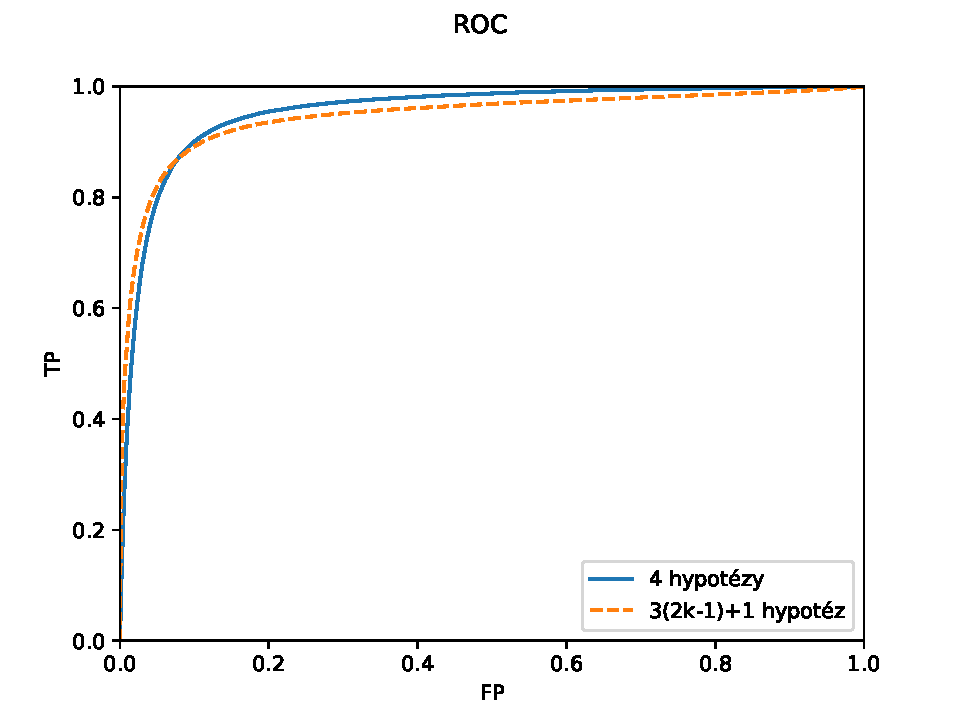
\includegraphics[width=.47\textwidth]{plots/1_ROC}\\
     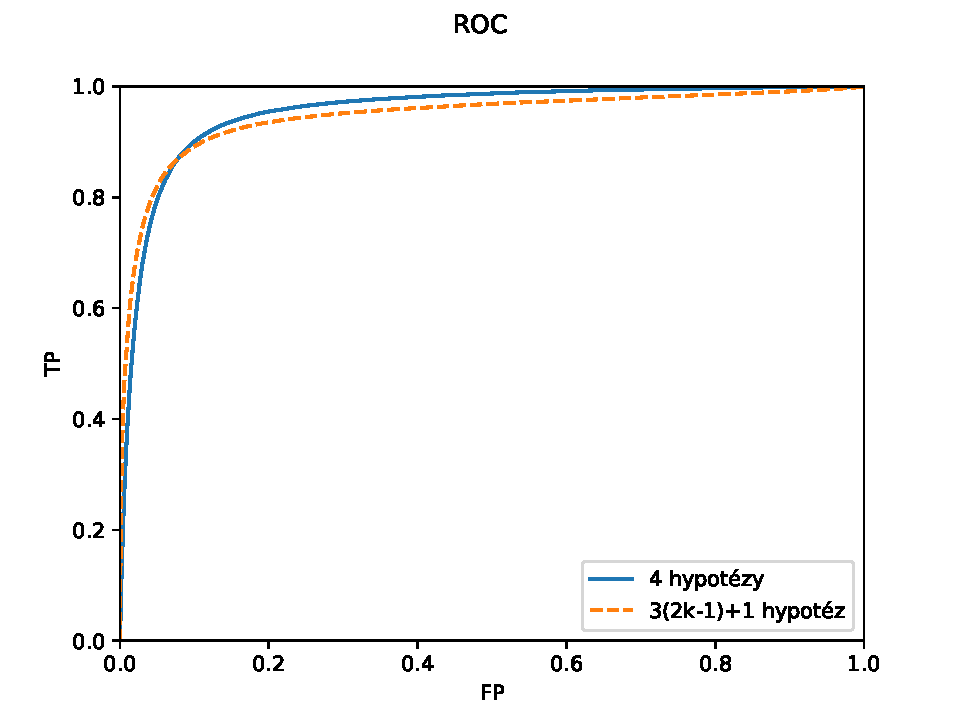
\includegraphics[width=.47\textwidth]{plots/1_ROC}\quad
     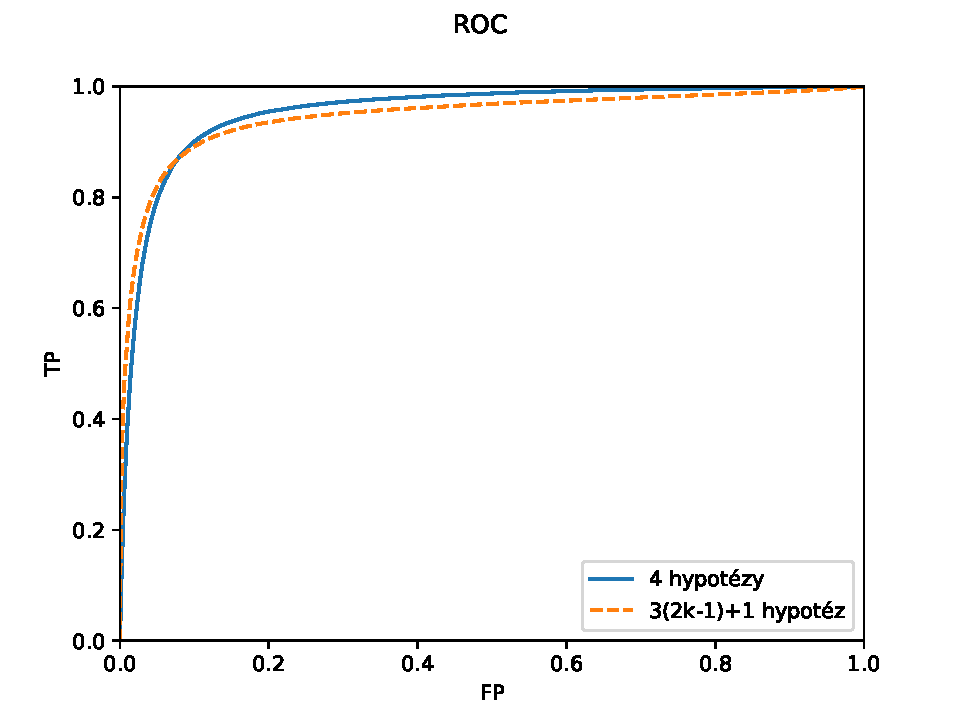
\includegraphics[width=.47\textwidth]{plots/1_ROC}\\
     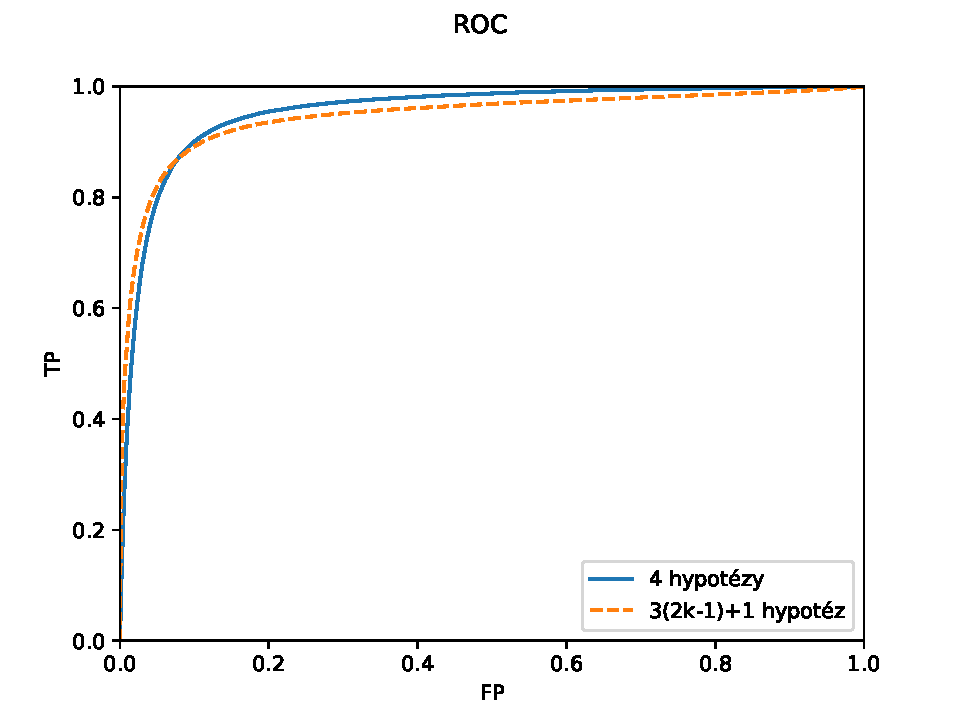
\includegraphics[width=.47\textwidth]{plots/1_ROC}\quad
     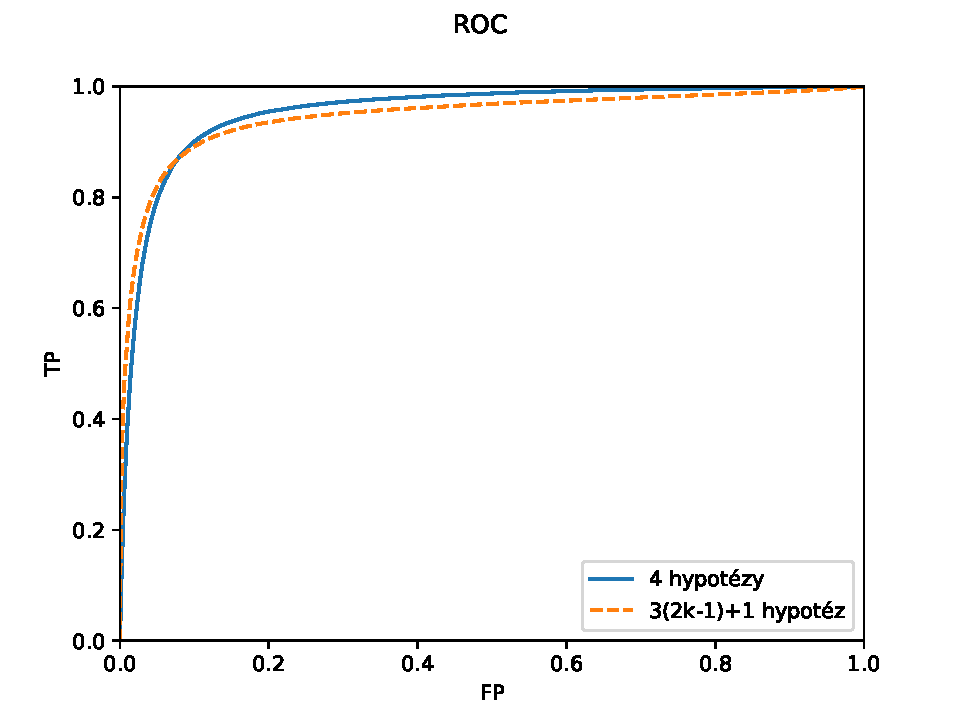
\includegraphics[width=.47\textwidth]{plots/1_ROC}\\
     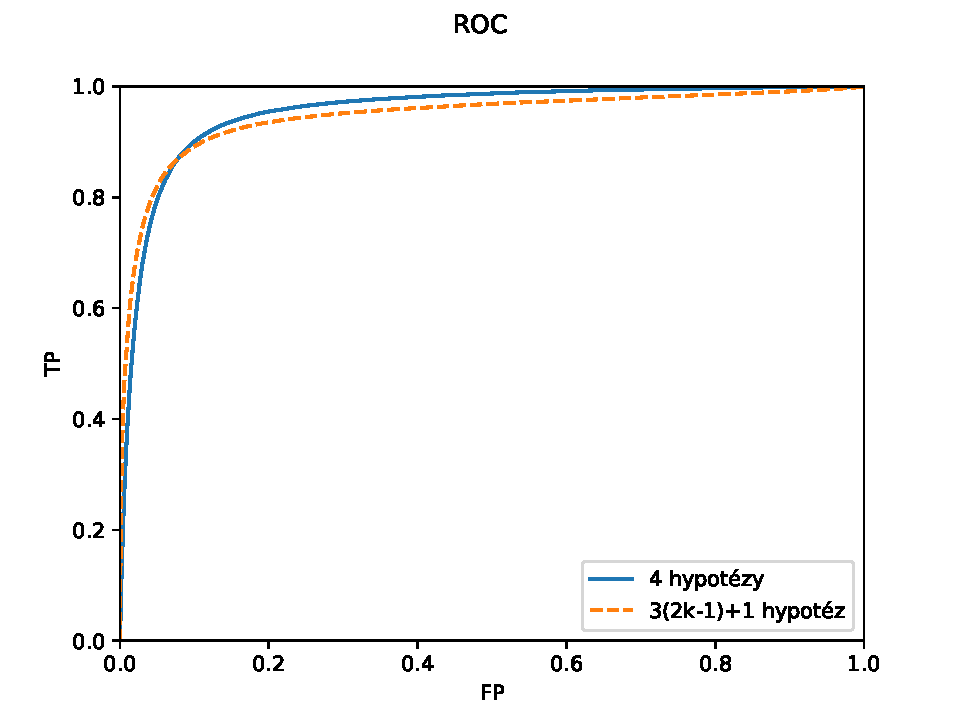
\includegraphics[width=.47\textwidth]{plots/1_ROC}\quad
     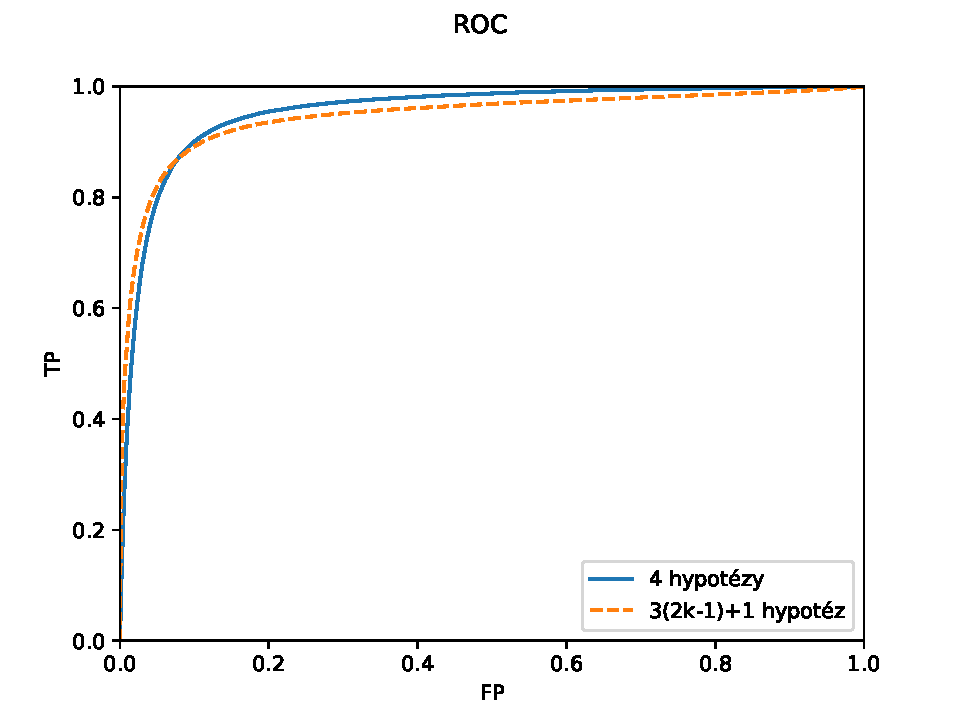
\includegraphics[width=.47\textwidth]{plots/1_ROC}
   \end{minipage}\\[1em]   
   \end{center}
\caption{Distribúcia úspešnosti identifikácie pre priamočiary prístup a pre náš model s $M=2$ a $M=3$.}
\label{fig:uspesnost_final}
\end{figure}


\begin{table}[]
\centering
\caption{Priemerná úspešnosť identifikácie pre priamočiary prístup a pre náš model s $M=2$ a $M=3$.}
\label{tab:uspesnost_final}
\begin{tabular}{llll}
\hline
testovacia sada & priamočiary prístup & $M=2$     & $M=3$     \\ \hline
KLEBS\_01       & $00,0 \%$           & $00,0 \%$ & $00,0 \%$ \\
KLEBS\_03       & $00,0 \%$           & $00,0 \%$ & $00,0 \%$ \\
KLEBS\_10       & $00,0 \%$           & $00,0 \%$ & $00,0 \%$ \\
KLEBS\_30       & $00,0 \%$           & $00,0 \%$ & $00,0 \%$ \\
NANO\_01        & $00,0 \%$           & $00,0 \%$ & $00,0 \%$ \\
NANO\_03        & $00,0 \%$           & $00,0 \%$ & $00,0 \%$ \\
NANO\_10        & $00,0 \%$           & $00,0 \%$ & $00,0 \%$ \\
NANO\_30        & $00,0 \%$           & $00,0 \%$ & $00,0 \%$
\end{tabular}
\end{table}

\todo{správne grafy a dáta v tabuľke}.